% answers.tex —— 2013 年·北京卷·理科 · 参考答案与详细解析片段
% 由 tools/generate_projects.py 依来源总账自 2013/2013_数学真题_北京理_试题.md + 2013/2013_数学真题_北京理_解析正文.md + 2013/2013_数学真题_北京理_答案要点.md 生成，勿手改（改源 MD 后重跑）


\begin{answer}
\gksolhead{1}{}

\textbf{题目}：

已知集合 $A=\{-1,0,1\}$，$B=\{x\mid-1\leqslant x<1\}$，则 $A\cap B=$\mbox{（　　）}

（A）$\{0\}$；（B）$\{-1,0\}$；（C）$\{0,1\}$；（D）$\{-1,0,1\}$。

\Needspace{4\baselineskip}
\textbf{解析}
\Needspace{5\baselineskip}
集合 $B$ 由满足 $-1\leqslant x<1$ 的实数组成。逐个数检验 $A$ 中的元素：
\nopagebreak[4]
\[-1\in B,\qquad 0\in B,\qquad 1\notin B\ (\text{\text{因为} }1<1\text{ \text{不成立}}).\]
\Needspace{5\baselineskip}
所以
\nopagebreak[4]
\[A\cap B=\{-1,0\}.\]
选 B。

\gkanswer{答案：B。$-1$，$0$ 在 $B$ 中而 $1\notin B$，故 $A\cap B=\{-1,0\}$。}

\end{answer}
\begin{answer}
\gksolhead{2}{}

\textbf{题目}：

在复平面内，复数 $(2-\mathrm i)^2$ 对应的点位于\mbox{（　　）}

（A）第一象限；（B）第二象限；（C）第三象限；（D）第四象限。

\Needspace{4\baselineskip}
\textbf{解析}
\Needspace{5\baselineskip}
由复数乘法，
\nopagebreak[4]
\[(2-\mathrm i)^2=4-4\mathrm i+\mathrm i^2=4-4\mathrm i-1=3-4\mathrm i.\]
其实部为 $3>0$，虚部为 $-4<0$，故对应点 $(3,-4)$ 位于第四象限。选 D。

\gkanswer{答案：D。$(2-\mathrm i)^2=3-4\mathrm i$，实部为正、虚部为负，对应点在第四象限。}

\end{answer}
\begin{answer}
\gksolhead{3}{}

\textbf{题目}：

“$\varphi=\pi$”是“曲线 $y=\sin(2x+\varphi)$ 过坐标原点”的\mbox{（　　）}

（A）充分而不必要条件；（B）必要而不充分条件；（C）充分必要条件；（D）既不充分也不必要条件。

\Needspace{4\baselineskip}
\textbf{解析}
\Needspace{5\baselineskip}
先看充分性。当 $\varphi=\pi$ 时，
\nopagebreak[4]
\[y=\sin(2x+\pi)=-\sin2x,\]
令 $x=0$ 得 $y=0$，曲线过坐标原点，故条件充分。

\Needspace{5\baselineskip}
再看必要性。若曲线过坐标原点，则
\nopagebreak[4]
\[\sin\varphi=0,\]
\Needspace{5\baselineskip}
即
\nopagebreak[4]
\[\varphi=k\pi\quad(k\in\mathbf Z),\]
并不一定有 $\varphi=\pi$，故条件不必要。

因此“$\varphi=\pi$”是“曲线过坐标原点”的充分而不必要条件。选 A。

\gkanswer{答案：A。$\varphi=\pi$ 时 $y=-\sin2x$ 过原点，充分；曲线过原点只要求 $\sin\varphi=0$，即 $\varphi=k\pi$，不必要。}

\end{answer}
\begin{answer}
\gksolhead{4}{}

\textbf{题目}：

执行如图所示的程序框图，输出的 $S$ 值为\mbox{（　　）}
\nopagebreak[4]
\begin{center}% 2013 年北京卷理科第 4 题：程序框图。
% 来源 PDF：普通高考/2013/2013北京理.pdf，第 1 页（印面 787）左栏。
% 流程：开始 → i=0,S=1 → S=(S^2+1)/(2S+1) → i=i+1 → i≥2?
%       是：输出 S → 结束；否：回到 S 赋值框。
\begin{tikzpicture}[font=\footnotesize, >=Stealth, line width=0.45pt,
  node distance=4.5mm,
  term/.style={draw, rounded corners=6pt, minimum height=1.8em, inner xsep=9pt},
  io/.style={draw, trapezium, trapezium left angle=70, trapezium right angle=110,
             minimum height=1.8em, inner xsep=6pt},
  box/.style={draw, minimum height=1.9em, inner xsep=6pt},
  dec/.style={draw, diamond, aspect=2.2, inner sep=1pt}]
  \node[term] (start) {开始};
  \node[box, below=4mm of start] (init) {$i=0$，$S=1$};
  \node[box, below=4mm of init] (assign) {$S=\dfrac{S^2+1}{2S+1}$};
  \node[box, below=4mm of assign] (inc) {$i=i+1$};
  \node[dec, below=5mm of inc] (cond) {$i\geqslant 2$};
  \node[io, right=16mm of cond] (output) {输出 $S$};
  \node[term, below=5mm of output] (end) {结束};
  \draw[->] (start) -- (init);
  \draw[->] (init) -- (assign);
  \draw[->] (assign) -- (inc);
  \draw[->] (inc) -- (cond);
  \draw[->] (cond) -- node[above] {是} (output);
  \draw[->] (output) -- (end);
  % 循环支路：从判断框左侧引出，向上回到 S 赋值框左侧
  \draw[->] (cond.west) -- node[above] {否} ++(-2.1,0) |- (assign.west);
\end{tikzpicture}
\end{center}
\nopagebreak[4]
（A）$1$；（B）$\dfrac23$；（C）$\dfrac{13}{21}$；（D）$\dfrac{610}{987}$。

\Needspace{4\baselineskip}
\textbf{解析}
初始 $i=0$，$S=1$。

\Needspace{5\baselineskip}
第一次执行循环体：
\nopagebreak[4]
\[S=\frac{1^2+1}{2\times1+1}=\frac23,\qquad i=1.\]
判断 $i\geqslant2$：因为 $1\geqslant2$ 不成立，回到循环体。

\Needspace{5\baselineskip}
第二次执行循环体：
\nopagebreak[4]
\[S=\frac{\left(\dfrac23\right)^2+1}{2\cdot\dfrac23+1}
=\frac{\dfrac49+1}{\dfrac43+1}
=\frac{\dfrac{13}9}{\dfrac73}
=\frac{13}9\cdot\frac37=\frac{13}{21},\qquad i=2.\]
\Needspace{5\baselineskip}
判断 $i\geqslant2$：因为 $2\geqslant2$ 成立，输出
\nopagebreak[4]
\[S=\frac{13}{21}.\]
选 C。

\gkanswer{答案：C。第一次循环得 $S=\dfrac23$，$i=1$ 不满足 $i\geqslant2$；第二次循环得 $S=\dfrac{13}{21}$，$i=2$ 满足，输出 $\dfrac{13}{21}$。}

\end{answer}
\begin{answer}
\gksolhead{5}{}

\textbf{题目}：

函数 $f(x)$ 的图象向右平移 $1$ 个单位长度，所得图象与曲线 $y=\mathrm e^x$ 关于 $y$ 轴对称，则 $f(x)=$\mbox{（　　）}

（A）$\mathrm e^{x+1}$；（B）$\mathrm e^{x-1}$；（C）$\mathrm e^{-x+1}$；（D）$\mathrm e^{-x-1}$。

\Needspace{4\baselineskip}
\textbf{解析}
\Needspace{5\baselineskip}
设平移后所得图象对应的函数为 $g(x)$。把 $f(x)$ 的图象向右平移 $1$ 个单位，得到
\nopagebreak[4]
\[g(x)=f(x-1).\]
\Needspace{5\baselineskip}
曲线 $y=\mathrm e^x$ 关于 $y$ 轴对称的曲线为 $y=\mathrm e^{-x}$，故
\nopagebreak[4]
\[f(x-1)=\mathrm e^{-x}.\]
\Needspace{5\baselineskip}
令 $t=x-1$，则 $x=t+1$，于是
\nopagebreak[4]
\[f(t)=\mathrm e^{-(t+1)}=\mathrm e^{-t-1},\]
\Needspace{5\baselineskip}
即
\nopagebreak[4]
\[f(x)=\mathrm e^{-x-1}.\]
选 D。

\gkanswer{答案：D。平移后图象为 $y=f(x-1)=\mathrm e^{-x}$，故 $f(x)=\mathrm e^{-(x+1)}=\mathrm e^{-x-1}$。}

\end{answer}
\begin{answer}
\gksolhead{6}{}

\textbf{题目}：

若双曲线 $\dfrac{x^2}{a^2}-\dfrac{y^2}{b^2}=1$ 的离心率为 $\sqrt3$，则其渐近线方程为\mbox{（　　）}

（A）$y=\pm2x$；（B）$y=\pm\sqrt2x$；（C）$y=\pm\dfrac12x$；（D）$y=\pm\dfrac{\sqrt2}2x$。

\Needspace{4\baselineskip}
\textbf{解析}
\Needspace{5\baselineskip}
双曲线的离心率满足
\nopagebreak[4]
\[e=\frac ca=\sqrt3,\]
\Needspace{5\baselineskip}
故
\nopagebreak[4]
\[c^2=3a^2.\]
\Needspace{5\baselineskip}
又
\nopagebreak[4]
\[b^2=c^2-a^2=3a^2-a^2=2a^2,\]
\Needspace{5\baselineskip}
所以
\nopagebreak[4]
\[\frac ba=\sqrt2.\]
\Needspace{5\baselineskip}
双曲线 $\dfrac{x^2}{a^2}-\dfrac{y^2}{b^2}=1$ 的渐近线为 $y=\pm\dfrac bax$，即
\nopagebreak[4]
\[y=\pm\sqrt2x.\]
选 B。

\gkanswer{答案：B。$c^2=3a^2$，$b^2=c^2-a^2=2a^2$，渐近线为 $y=\pm\dfrac bax=\pm\sqrt2x$。}

\end{answer}
\begin{answer}
\gksolhead{7}{}

\textbf{题目}：

直线 $l$ 过抛物线 $C:x^2=4y$ 的焦点且与 $y$ 轴垂直，则 $l$ 与 $C$ 所围成的图形的面积等于\mbox{（　　）}

（A）$\dfrac43$；（B）$2$；（C）$\dfrac83$；（D）$\dfrac{16\sqrt2}3$。

\Needspace{4\baselineskip}
\textbf{解析}
\Needspace{5\baselineskip}
抛物线 $x^2=4y$ 的焦点为 $(0,1)$。直线 $l$ 过焦点且与 $y$ 轴垂直，故
\nopagebreak[4]
\[l:y=1.\]
\Needspace{5\baselineskip}
由
\nopagebreak[4]
\[\begin{cases}y=1,\\x^2=4y\end{cases}\]
得 $x^2=4$，即 $x=\pm2$，两交点为 $(-2,1)$，$(2,1)$。

\Needspace{5\baselineskip}
在 $[-2,2]$ 上抛物线位于直线下方，所求面积为
\nopagebreak[4]
\[\begin{aligned}
S&=\int_{-2}^{2}\left(1-\frac{x^2}4\right)\mathrm dx\\
&=\left[x-\frac{x^3}{12}\right]_{-2}^{2}\\
&=\left(2-\frac{8}{12}\right)-\left(-2+\frac{8}{12}\right)\\
&=\frac83.
\end{aligned}\]
选 C。

\gkanswer{答案：C。焦点为 $(0,1)$，$l:y=1$ 与 $C$ 交于 $(\pm2,1)$，面积为 $\displaystyle\int_{-2}^{2}\left(1-\dfrac{x^2}4\right)\mathrm dx=\dfrac83$。}

\end{answer}
\begin{answer}
\gksolhead{8}{}

\textbf{题目}：

\Needspace{5\baselineskip}
设关于 $x$，$y$ 的不等式组
\nopagebreak[4]
\[\begin{cases}2x-y+1\geqslant0,\\ x+m<0,\\ y-m>0\end{cases}\]
表示的平面区域内存在点 $P(x_0,y_0)$，满足 $x_0-2y_0=2$，则 $m$ 的取值范围是\mbox{（　　）}

（A）$\left(-\infty,\dfrac43\right)$；（B）$\left(-\infty,\dfrac13\right)$；（C）$\left(-\infty,-\dfrac23\right)$；（D）$\left(-\infty,-\dfrac53\right)$。

\Needspace{4\baselineskip}
\textbf{解析}
\Needspace{5\baselineskip}
题设区域由三条边界围成：
\nopagebreak[4]
\[y\leqslant2x+1,\qquad x<-m,\qquad y>m.\]
\Needspace{5\baselineskip}
条件 $x_0-2y_0=2$ 即
\nopagebreak[4]
\[y_0=\frac{x_0}2-1.\]
\Needspace{5\baselineskip}
点 $P$ 在区域内，等价于同时成立
\nopagebreak[4]
\[\frac{x_0}2-1\leqslant2x_0+1,\qquad x_0<-m,\qquad \frac{x_0}2-1>m.\]
\Needspace{5\baselineskip}
第一式化为
\nopagebreak[4]
\[-2\leqslant\frac32x_0,\qquad x_0\geqslant-\frac43;\]
\Needspace{5\baselineskip}
第三式化为
\nopagebreak[4]
\[x_0>2m+2.\]
\Needspace{5\baselineskip}
于是问题等价于：存在 $x_0$ 同时满足
\nopagebreak[4]
\[x_0\geqslant-\frac43,\qquad x_0>2m+2,\qquad x_0<-m,\]
\Needspace{5\baselineskip}
即区间
\nopagebreak[4]
\[\left(\max\left\{2m+2,-\frac43\right\},\ -m\right)\]
\Needspace{5\baselineskip}
非空。这要求
\nopagebreak[4]
\[-m>\max\left\{2m+2,-\frac43\right\}.\]
\Needspace{5\baselineskip}
由 $-m>2m+2$ 得
\nopagebreak[4]
\[m<-\frac23.\]
\Needspace{5\baselineskip}
当 $m<-\dfrac23$ 时，$-m>\dfrac23>-\dfrac43$，即 $-m>-\dfrac43$ 也成立，故上面的区间确实非空。所以 $m$ 的取值范围是
\nopagebreak[4]
\[\left(-\infty,-\frac23\right).\]
选 C。

\gkanswer{答案：C。把 $y_0=\dfrac{x_0}2-1$ 代入三条约束，等价于存在 $x_0$ 满足 $\max\{2m+2,-\dfrac43\}<x_0<-m$，故 $m<-\dfrac23$。}

\end{answer}
\begin{answer}
\gksolhead{9}{}

\textbf{题目}：

在极坐标系中，点 $\left(2,\dfrac{\pi}6\right)$ 到直线 $\rho\sin\theta=2$ 的距离等于\gkblank{}。

\Needspace{4\baselineskip}
\textbf{解析}
\Needspace{5\baselineskip}
极坐标点 $\left(2,\dfrac{\pi}6\right)$ 的直角坐标为
\nopagebreak[4]
\[x=2\cos\frac{\pi}6=\sqrt3,\qquad y=2\sin\frac{\pi}6=1.\]
\Needspace{5\baselineskip}
直线 $\rho\sin\theta=2$ 即
\nopagebreak[4]
\[y=2.\]
\Needspace{5\baselineskip}
点 $(\sqrt3,1)$ 到直线 $y=2$ 的距离为
\nopagebreak[4]
\[d=|1-2|=1.\]
填 $1$。

\gkanswer{答案：$1$。点的直角坐标为 $(\sqrt3,1)$，直线为 $y=2$，距离为 $|1-2|=1$。}

\end{answer}
\begin{answer}
\gksolhead{10}{}

\textbf{题目}：

若等比数列 $\{a_n\}$ 满足 $a_2+a_4=20$，$a_3+a_5=40$，则公比 $q=$\gkblank{}，前 $n$ 项和 $S_n=$\gkblank{}。

\Needspace{4\baselineskip}
\textbf{解析}
\Needspace{5\baselineskip}
设公比为 $q$。由
\nopagebreak[4]
\[a_3+a_5=q(a_2+a_4)\]
\Needspace{5\baselineskip}
得
\nopagebreak[4]
\[40=20q,\qquad q=2.\]
\Needspace{5\baselineskip}
再由
\nopagebreak[4]
\[a_2+a_4=a_1q+a_1q^3=a_1(2+8)=10a_1=20\]
\Needspace{5\baselineskip}
得
\nopagebreak[4]
\[a_1=2.\]
\Needspace{5\baselineskip}
所以
\nopagebreak[4]
\[S_n=\frac{a_1(1-q^n)}{1-q}=\frac{2(2^n-1)}{2-1}=2^{n+1}-2.\]
填 $q=2$，$S_n=2^{n+1}-2$。

\gkanswer{答案：$q=2$，$S_n=2^{n+1}-2$。由 $a_3+a_5=q(a_2+a_4)$ 得 $q=2$；再由 $a_2+a_4=10a_1=20$ 得 $a_1=2$。}

\end{answer}
\begin{answer}
\gksolhead{11}{}

\textbf{题目}：

如图，$AB$ 为圆 $O$ 的直径，$PA$ 为圆 $O$ 的切线，$PB$ 与圆 $O$ 相交于 $D$，若 $PA=3$，$PD:DB=9:16$，则 $PD=$\gkblank{}，$AB=$\gkblank{}。
\nopagebreak[4]
\begin{center}% 2013 年北京卷理科第 11 题：圆的切线与割线。
% 来源 PDF：普通高考/2013/2013北京理.pdf，第 1 页（印面 787）中栏。
% AB 为圆 O 的直径，PA 切圆于 A，PB 与圆交于 D；PA=3，PD:DB=9:16。
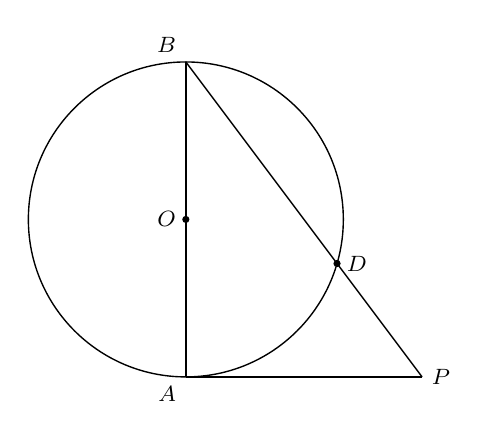
\begin{tikzpicture}[font=\footnotesize, line width=0.5pt, scale=1]
  \coordinate (O) at (0,0);
  \coordinate (A) at (0,-2);
  \coordinate (B) at (0,2);
  \coordinate (P) at (3,-2);
  \coordinate (D) at (1.92,-0.56);
  % 圆
  \draw (O) circle (2);
  % 直径 AB
  \draw (A) -- (B);
  % 切线 PA 与割线 PB
  \draw (P) -- (A);
  \draw (P) -- (B);
  % 点
  \fill (O) circle (1.3pt);
  \fill (D) circle (1.3pt);
  \node[left] at (O) {$O$};
  \node[below left] at (A) {$A$};
  \node[above left] at (B) {$B$};
  \node[right] at (P) {$P$};
  \node[right] at (D) {$D$};
\end{tikzpicture}
\end{center}
\nopagebreak[4]
\Needspace{4\baselineskip}
\textbf{解析}
\Needspace{5\baselineskip}
由切割线定理，
\nopagebreak[4]
\[PA^2=PD\cdot PB.\]
\Needspace{5\baselineskip}
设 $PD=9k$，$DB=16k$（$k>0$），则
\nopagebreak[4]
\[PB=PD+DB=25k.\]
\Needspace{5\baselineskip}
代入 $PA=3$：
\nopagebreak[4]
\[9=9k\cdot25k=225k^2,\]
\Needspace{5\baselineskip}
解得
\nopagebreak[4]
\[k=\frac15,\]
\Needspace{5\baselineskip}
故
\nopagebreak[4]
\[PD=9k=\frac95,\qquad PB=25k=5.\]
\Needspace{5\baselineskip}
因为 $AB$ 是直径，$PA$ 切圆于 $A$，所以
\nopagebreak[4]
\[PA\perp AB.\]
\Needspace{5\baselineskip}
在直角三角形 $PAB$ 中，
\nopagebreak[4]
\[AB=\sqrt{PB^2-PA^2}=\sqrt{25-9}=4.\]
填 $PD=\dfrac95$，$AB=4$。

\gkanswer{答案：$PD=\dfrac95$，$AB=4$。切割线定理给出 $PA^2=PD\cdot PB$，设 $PD=9k$，$DB=16k$，得 $k=\dfrac15$；又 $PA\perp AB$，故 $AB=\sqrt{PB^2-PA^2}=4$。}

\end{answer}
\begin{answer}
\gksolhead{12}{}

\textbf{题目}：

将序号分别为 $1$，$2$，$3$，$4$，$5$ 的 $5$ 张参观券全部分给 $4$ 人，每人至少 $1$ 张，如果分给同一人的 $2$ 张参观券连号，那么不同的分法种数是\gkblank{}。

\Needspace{4\baselineskip}
\textbf{解析}
每人至少 $1$ 张，而参观券共 $5$ 张、分给 $4$ 人，故必有一人得 $2$ 张，其余三人各得 $1$ 张。

\Needspace{5\baselineskip}
分给同一人的 $2$ 张必须连号，连号的两张只能是
\nopagebreak[4]
\[\{1,2\},\ \{2,3\},\ \{3,4\},\ \{4,5\},\]
共 $4$ 种选法。

\Needspace{5\baselineskip}
选定连号的两张后，把“这两张”与其余 $3$ 张看作 $4$ 组，分给 $4$ 个不同的人，有
\nopagebreak[4]
\[4!=24\]
种分法。

\Needspace{5\baselineskip}
所以不同的分法种数为
\nopagebreak[4]
\[4\times4!=96.\]
填 $96$。

\gkanswer{答案：$96$。连号的 $2$ 张有 $4$ 种选法，与其余 $3$ 张一起分给 $4$ 人有 $4!$ 种，共 $4\times4!=96$ 种。}

\end{answer}
\begin{answer}
\gksolhead{13}{}

\textbf{题目}：

向量 $\boldsymbol a$，$\boldsymbol b$，$\boldsymbol c$ 在正方形网格中的位置如图所示，若 $\boldsymbol c=\lambda\boldsymbol a+\mu\boldsymbol b$（$\lambda$，$\mu\in\mathbf R$），则 $\dfrac{\lambda}{\mu}=$\gkblank{}。
\nopagebreak[4]
\begin{center}% 2013 年北京卷理科第 13 题：正方形网格中的向量 a，b，c。
% 来源 PDF：普通高考/2013/2013北京理.pdf，第 1 页（印面 787）中栏。
% 网格 8×4；a 由 (2,0) 指向 (1,1)，b 由 (1,1) 指向 (7,3)，
% c 由 (7,3) 指向 (6,0)，故 a=(-1,1)，b=(6,2)，c=(-1,-3)。
\begin{tikzpicture}[font=\footnotesize, line width=0.4pt, scale=0.62]
  % 正方形网格
  \draw[step=1, gray!70] (0,0) grid (8,4);
  \draw[line width=0.6pt] (0,0) rectangle (8,4);
  % 向量 b
  \draw[->, line width=1.1pt, >=Stealth] (1,1) -- (7,3);
  % 向量 a
  \draw[->, line width=1.1pt, >=Stealth] (2,0) -- (1,1);
  % 向量 c
  \draw[->, line width=1.1pt, >=Stealth] (7,3) -- (6,0);
  % 标签
  \node at (0.92,0.62) {$a$};
  \node[above] at (4.1,2.35) {$b$};
  \node[right] at (6.62,1.45) {$c$};
\end{tikzpicture}
\end{center}
\nopagebreak[4]
\Needspace{4\baselineskip}
\textbf{解析}
\Needspace{5\baselineskip}
以正方形网格的两条边为坐标轴建立坐标系，每个小方格边长为 $1$。按图中箭头的起点与终点读出
\nopagebreak[4]
\[\boldsymbol a=(-1,1),\qquad \boldsymbol b=(6,2),\qquad \boldsymbol c=(-1,-3).\]
\Needspace{5\baselineskip}
由 $\boldsymbol c=\lambda\boldsymbol a+\mu\boldsymbol b$ 得
\nopagebreak[4]
\[\begin{cases}-\lambda+6\mu=-1,\\ \lambda+2\mu=-3.\end{cases}\]
\Needspace{5\baselineskip}
两式相加：
\nopagebreak[4]
\[8\mu=-4,\qquad \mu=-\frac12.\]
\Needspace{5\baselineskip}
代入第二式：
\nopagebreak[4]
\[\lambda=-3-2\mu=-3+1=-2.\]
\Needspace{5\baselineskip}
所以
\nopagebreak[4]
\[\frac{\lambda}{\mu}=\frac{-2}{-\dfrac12}=4.\]
填 $4$。

\gkanswer{答案：$4$。取网格坐标得 $\boldsymbol a=(-1,1)$，$\boldsymbol b=(6,2)$，$\boldsymbol c=(-1,-3)$，解得 $\lambda=-2$，$\mu=-\dfrac12$，故 $\dfrac{\lambda}{\mu}=4$。}

\end{answer}
\begin{answer}
\gksolhead{14}{}

\textbf{题目}：

如图，在棱长为 $2$ 的正方体 $ABCD-A_1B_1C_1D_1$ 中，$E$ 为 $BC$ 的中点，点 $P$ 在线段 $D_1E$ 上，点 $P$ 到直线 $CC_1$ 的距离的最小值为\gkblank{}。
\nopagebreak[4]
\begin{center}% 2013 年北京卷理科第 14 题：棱长为 2 的正方体 ABCD-A1B1C1D1。
% 来源 PDF：普通高考/2013/2013北京理.pdf，第 1 页（印面 787）中栏。
% E 为 BC 的中点，P 在线段 D1E 上。
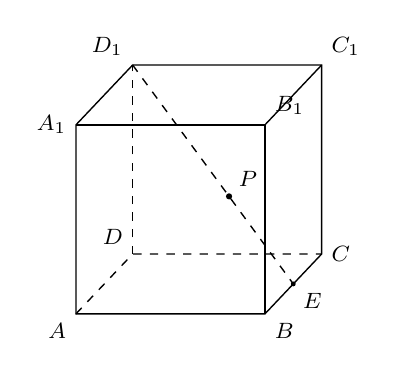
\begin{tikzpicture}[font=\footnotesize, line width=0.5pt, scale=0.8]
  % 前面 ABB1A1
  \coordinate (A) at (0,0);
  \coordinate (B) at (3,0);
  \coordinate (A1) at (0,3);
  \coordinate (B1) at (3,3);
  % 后面 DCC1D1（斜二测方向）
  \coordinate (D) at (0.9,0.95);
  \coordinate (C) at (3.9,0.95);
  \coordinate (C1) at (3.9,3.95);
  \coordinate (D1) at (0.9,3.95);
  % E 为 BC 中点
  \coordinate (E) at (3.45,0.475);
  % P 在线段 D1E 上
  \coordinate (P) at (2.43,1.865);
  % 可见棱
  \draw (A) -- (B) -- (C) -- (C1) -- (D1) -- (A1) -- cycle;
  \draw (A1) -- (B1) -- (B);
  \draw (B1) -- (C1);
  \draw (C) -- (C1);
  % 被遮挡的棱
  \draw[dashed] (A) -- (D) -- (C);
  \draw[dashed] (D) -- (D1);
  % 线段 D1E 与点 P
  \draw[dashed] (D1) -- (E);
  \fill (P) circle (1.4pt);
  \fill (E) circle (1.1pt);
  % 标签
  \node[below left] at (A) {$A$};
  \node[below right] at (B) {$B$};
  \node[right] at (C) {$C$};
  \node[above left] at (D) {$D$};
  \node[left] at (A1) {$A_1$};
  \node[above right] at (B1) {$B_1$};
  \node[above right] at (C1) {$C_1$};
  \node[above left] at (D1) {$D_1$};
  \node[below right] at (E) {$E$};
  \node[above right] at (P) {$P$};
\end{tikzpicture}
\end{center}
\nopagebreak[4]
\Needspace{4\baselineskip}
\textbf{解析}
\Needspace{5\baselineskip}
以 $A$ 为原点，$AB$，$AD$，$AA_1$ 所在直线分别为 $x$，$y$，$z$ 轴建立空间直角坐标系。棱长为 $2$，则
\nopagebreak[4]
\[D_1(0,2,2),\qquad B(2,0,0),\qquad C(2,2,0),\qquad C_1(2,2,2).\]
\Needspace{5\baselineskip}
$E$ 为 $BC$ 的中点，故
\nopagebreak[4]
\[E(2,1,0).\]
\Needspace{5\baselineskip}
点 $P$ 在线段 $D_1E$ 上，可设
\nopagebreak[4]
\[\overrightarrow{D_1P}=t\overrightarrow{D_1E},\qquad 0\leqslant t\leqslant1,\]
\Needspace{5\baselineskip}
即
\nopagebreak[4]
\[P(2t,\,2-t,\,2-2t).\]
\Needspace{5\baselineskip}
直线 $CC_1$ 是过 $(2,2,0)$ 且平行于 $z$ 轴的直线。点 $P$ 到 $CC_1$ 的距离等于 $P$ 在 $xOy$ 平面上的投影 $(2t,2-t)$ 到 $(2,2)$ 的距离：
\nopagebreak[4]
\[\begin{aligned}
d^2&=(2t-2)^2+(2-t-2)^2\\
&=(2-2t)^2+t^2\\
&=5t^2-8t+4.
\end{aligned}\]
\Needspace{5\baselineskip}
这是关于 $t$ 的二次函数，在
\nopagebreak[4]
\[t=\frac{8}{2\times5}=\frac45\]
\Needspace{5\baselineskip}
处取得最小值，且 $\dfrac45\in[0,1]$。此时
\nopagebreak[4]
\[d^2=5\cdot\frac{16}{25}-8\cdot\frac45+4=\frac{16}5-\frac{32}5+\frac{20}5=\frac45,\]
\Needspace{5\baselineskip}
故
\nopagebreak[4]
\[d_{\min}=\frac{2}{\sqrt5}=\frac{2\sqrt5}5.\]
填 $\dfrac{2\sqrt5}5$。

\gkanswer{答案：$\dfrac{2\sqrt5}5$。建系得 $P(2t,2-t,2-2t)$，到直线 $CC_1$ 的距离为 $\sqrt{5t^2-8t+4}$，在 $t=\dfrac45$ 处取最小值 $\dfrac{2\sqrt5}5$。}

\end{answer}
\begin{answer}
\gksolhead{15}{}

\textbf{题目}：

在 $\triangle ABC$ 中，$a=3$，$b=2\sqrt6$，$\angle B=2\angle A$。

（1） 求 $\cos A$ 的值；

（2） 求 $c$ 的值。

\Needspace{4\baselineskip}
\textbf{解析}
\Needspace{5\baselineskip}
\textbf{（1）} 由正弦定理，
\nopagebreak[4]
\[\frac{a}{\sin A}=\frac{b}{\sin B}.\]
\Needspace{5\baselineskip}
因为 $\angle B=2\angle A$，所以
\nopagebreak[4]
\[\frac{3}{\sin A}=\frac{2\sqrt6}{\sin2A}=\frac{2\sqrt6}{2\sin A\cos A}.\]
\Needspace{5\baselineskip}
约去 $\sin A>0$，得
\nopagebreak[4]
\[3=\frac{\sqrt6}{\cos A},\]
\Needspace{5\baselineskip}
即
\nopagebreak[4]
\[\cos A=\frac{\sqrt6}{3}.\]

\Needspace{5\baselineskip}
\textbf{（2）} 由（1），
\nopagebreak[4]
\[\sin A=\sqrt{1-\cos^2A}=\sqrt{1-\frac23}=\frac{\sqrt3}3,\]
\nopagebreak[4]
\[\cos B=\cos2A=2\cos^2A-1=2\cdot\frac23-1=\frac13,\]
\nopagebreak[4]
\[\sin B=\sqrt{1-\frac19}=\frac{2\sqrt2}3.\]
\Needspace{5\baselineskip}
因为 $C=\pi-(A+B)$，所以
\nopagebreak[4]
\[\sin C=\sin(A+B)=\sin A\cos B+\cos A\sin B
=\frac{\sqrt3}3\cdot\frac13+\frac{\sqrt6}3\cdot\frac{2\sqrt2}3
=\frac{\sqrt3}9+\frac{4\sqrt3}9=\frac{5\sqrt3}9.\]
\Needspace{5\baselineskip}
由正弦定理，
\nopagebreak[4]
\[c=\frac{a\sin C}{\sin A}=\frac{3\cdot\dfrac{5\sqrt3}9}{\dfrac{\sqrt3}3}=3\cdot\frac{5\sqrt3}9\cdot\frac{3}{\sqrt3}=5.\]

\gkanswer{答案（1）：$\dfrac{\sqrt6}3$。由正弦定理及 $\angle B=2\angle A$ 得 $3=2\sqrt6\cdot\dfrac{\sin A}{\sin2A}=\dfrac{\sqrt6}{\cos A}$。}

\gkanswer{答案（2）：$5$。$\cos B=\dfrac13$，$\sin B=\dfrac{2\sqrt2}3$，$\sin C=\sin(A+B)=\dfrac{5\sqrt3}9$，故 $c=\dfrac{a\sin C}{\sin A}=5$。}

\end{answer}
\begin{answer}
\gksolhead{16}{}

\textbf{题目}：

下图是某市 $3$ 月 $1$ 日至 $14$ 日的空气质量指数趋势图，空气质量指数小于 $100$ 表示空气质量优良，空气质量指数大于 $200$ 表示空气重度污染。某人随机选择 $3$ 月 $1$ 日至 $3$ 月 $13$ 日中的某一天到达该市，并停留 $2$ 天。
\nopagebreak[4]
\begin{center}% 2013 年北京卷理科第 16 题：3 月 1 日至 14 日空气质量指数趋势图。
% 来源 PDF：普通高考/2013/2013北京理.pdf，第 1 页（印面 787）右栏。
% 14 个数据点（600 dpi 原页逐个核对）：86，25，57，143，220，160，40，
% 217，160，121，158，86，79，37。
\begin{tikzpicture}[font=\scriptsize, >=Stealth, line width=0.45pt,
  x=0.79cm, y=0.026cm]
  % 坐标轴
  \draw[->] (0,0) -- (14.7,0);
  \node[below right] at (14.7,0) {日期};
  \draw[->] (0,0) -- (0,285) node[above] {空气质量指数};
  % 纵轴刻度与虚线
  \foreach \y in {50,100,150,200,250} {
    \draw (0,\y) -- (-0.12,\y) node[left] {\y};
    \draw[dashed, gray!55] (0,\y) -- (14.55,\y);
  }
  \node[below left] at (0,0) {$0$};
  % 横轴日期
  \foreach \i in {1,...,14} \node[below, font=\tiny] at (\i,0) {\i 日};
  % 数据折线与数据点
  \foreach \i/\v in {1/86,2/25,3/57,4/143,5/220,6/160,7/40,
                     8/217,9/160,10/121,11/158,12/86,13/79,14/37}
    \fill (\i,\v) circle (1.2pt);
  \draw (1,86) -- (2,25) -- (3,57) -- (4,143) -- (5,220) -- (6,160)
        -- (7,40) -- (8,217) -- (9,160) -- (10,121) -- (11,158)
        -- (12,86) -- (13,79) -- (14,37);
  % 数值标注
  \node[above left] at (1,86) {86};
  \node[left] at (2,25) {25};
  \node[above left] at (3,57) {57};
  \node[above] at (4,143) {143};
  \node[left] at (5,220) {220};
  \node[above left] at (6,160) {160};
  \node[above left] at (7,40) {40};
  \node[right] at (8,217) {217};
  \node[above left] at (9,160) {160};
  \node[left] at (10,121) {121};
  \node[above] at (11,158) {158};
  \node[below left] at (12,86) {86};
  \node[right] at (13,79) {79};
  \node[above left] at (14,37) {37};
\end{tikzpicture}
\end{center}
\nopagebreak[4]
（1） 求此人到达当日空气重度污染的概率；

（2） 设 $X$ 是此人停留期间空气质量优良的天数，求 $X$ 的分布列与数学期望；

（3） 由图判断从哪天开始连续三天的空气质量指数方差最大？（结论不要求证明）

\Needspace{4\baselineskip}
\textbf{解析}
\Needspace{5\baselineskip}
由趋势图读出 $3$ 月 $1$ 日至 $14$ 日的空气质量指数依次为
\nopagebreak[4]
\[86,\ 25,\ 57,\ 143,\ 220,\ 160,\ 40,\ 217,\ 160,\ 121,\ 158,\ 86,\ 79,\ 37.\]
其中小于 $100$ 的日期为 $1$，$2$，$3$，$7$，$12$，$13$，$14$ 日；大于 $200$ 的日期为 $5$，$8$ 日。

\Needspace{5\baselineskip}
\textbf{（1）} 到达日期在 $3$ 月 $1$ 日至 $13$ 日中等可能选取，共 $13$ 种。到达当日为重度污染，只有第 $5$ 日（$220$）与第 $8$ 日（$217$）两种，故所求概率为
\nopagebreak[4]
\[P=\frac{2}{13}.\]

\textbf{（2）} 设到达日为第 $i$ 日（$i=1,2,\cdots,13$），停留的两天为第 $i$ 日与第 $i+1$ 日。逐日统计其中空气质量优良的天数：

\begin{center}
\begin{tabular}{lll}
\toprule
$i$ & 两日指数 & $X$ \\
\midrule
1 & 86，25 & 2 \\
2 & 25，57 & 2 \\
3 & 57，143 & 1 \\
4 & 143，220 & 0 \\
5 & 220，160 & 0 \\
6 & 160，40 & 1 \\
7 & 40，217 & 1 \\
8 & 217，160 & 0 \\
9 & 160，121 & 0 \\
10 & 121，158 & 0 \\
11 & 158，86 & 1 \\
12 & 86，79 & 2 \\
13 & 79，37 & 2 \\
\bottomrule
\end{tabular}
\end{center}

\Needspace{5\baselineskip}
$X=0$ 有 $i=4,5,8,9,10$ 共 $5$ 天；$X=1$ 有 $i=3,6,7,11$ 共 $4$ 天；$X=2$ 有 $i=1,2,12,13$ 共 $4$ 天。所以 $X$ 的分布列为
\nopagebreak[4]
\[P(X=0)=\frac5{13},\qquad P(X=1)=\frac4{13},\qquad P(X=2)=\frac4{13}.\]
\Needspace{5\baselineskip}
数学期望为
\nopagebreak[4]
\[E(X)=0\cdot\frac5{13}+1\cdot\frac4{13}+2\cdot\frac4{13}=\frac{12}{13}.\]

\Needspace{5\baselineskip}
\textbf{（3）} 设从第 $i$ 日开始的连续三天指数为 $x_i$，$x_{i+1}$，$x_{i+2}$，其方差为
\nopagebreak[4]
\[s_i^2=\frac13\sum_{k=0}^{2}\left(x_{i+k}-\bar x_i\right)^2,\qquad \bar x_i=\frac{x_i+x_{i+1}+x_{i+2}}3.\]
逐一计算 $i=1,2,\cdots,12$：

\begin{center}
\begin{tabular}{lll}
\toprule
起始日 & 三天指数 & 方差 \\
\midrule
1 & 86，25，57 & 620.7 \\
2 & 25，57，143 & 2482.7 \\
3 & 57，143，220 & 4432.7 \\
4 & 143，220，160 & 1090.9 \\
5 & 220，160，40 & 5600.0 \\
6 & 160，40，217 & 5442.0 \\
7 & 40，217，160 & 5442.0 \\
8 & 217，160，121 & 1554.0 \\
9 & 160，121，158 & 321.6 \\
10 & 121，158，86 & 864.2 \\
11 & 158，86，79 & 1274.9 \\
12 & 86，79，37 & 468.2 \\
\bottomrule
\end{tabular}
\end{center}

其中以 $i=5$ 的方差 $5600$ 最大。故从 $5$ 日开始连续三天的空气质量指数方差最大。

\gkanswer{答案（1）：$\dfrac2{13}$。$3$ 月 $1$ 日至 $13$ 日中等概率选一天，到达当日重度污染只有 $5$ 日与 $8$ 日两天。}

\gkanswer{答案（2）：$P(X=0)=\dfrac5{13}$，$P(X=1)=\dfrac4{13}$，$P(X=2)=\dfrac4{13}$，$E(X)=\dfrac{12}{13}$。逐日检查相邻两天中空气质量优良的天数即得。}

\gkanswer{答案（3）：从 $5$ 日开始。三天 $220$，$160$，$40$ 的方差为 $5600$，大于其余各起始日对应的方差。}

\end{answer}
\begin{answer}
\gksolhead{17}{}

\textbf{题目}：

如图，在三棱柱 $ABC-A_1B_1C_1$ 中，$AA_1C_1C$ 是边长为 $4$ 的正方形。平面 $ABC\perp$ 平面 $AA_1C_1C$，$AB=3$，$BC=5$。

（1） 求证：$AA_1\perp$ 平面 $ABC$；

（2） 求二面角 $A_1-BC_1-B_1$ 的余弦值；

（3） 证明：在线段 $BC_1$ 上存在点 $D$，使得 $AD\perp A_1B$，并求 $\dfrac{BD}{BC_1}$ 的值。
\nopagebreak[4]
\begin{center}% 2013 年北京卷理科第 17 题：三棱柱 ABC-A1B1C1。
% 来源 PDF：普通高考/2013/2013北京理.pdf，第 2 页（印面 788）左栏。
% AA1C1C 是边长为 4 的正方形，平面 ABC⊥平面 AA1C1C，AB=3，BC=5。
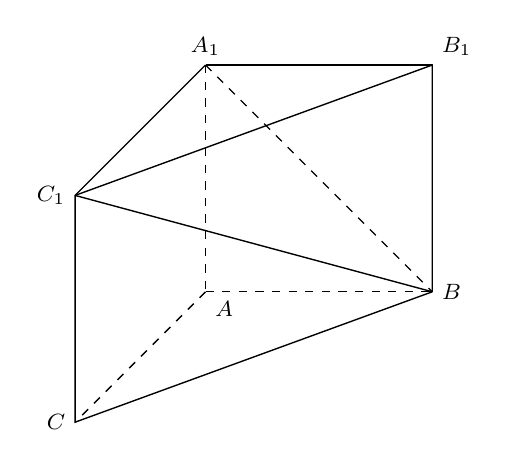
\begin{tikzpicture}[font=\footnotesize, line width=0.5pt, scale=0.72]
  % 正方形侧面 AA1C1C（平行四边形画法）：A1 在上，C1 在左上，A 在下，C 在左下
  \coordinate (A1) at (0,0);
  \coordinate (C1) at (-2.3,-2.3);
  \coordinate (A)  at (0,-4.0);
  \coordinate (C)  at (-2.3,-6.3);
  % AB 垂直于侧面，B 在右前方
  \coordinate (B)  at (4.0,-4.0);
  \coordinate (B1) at (4.0,0);
  % 可见棱
  \draw (A1) -- (C1) -- (C) -- (B);
  \draw (C1) -- (B1) -- (B);
  \draw (A1) -- (B1);
  % 被遮挡的棱
  \draw[dashed] (A1) -- (A);
  \draw[dashed] (A) -- (C);
  \draw[dashed] (A) -- (B);
  % 辅助线 A1B、C1B
  \draw[dashed] (A1) -- (B);
  \draw (C1) -- (B);
  % 顶点标签
  \node[above] at (A1) {$A_1$};
  \node[left] at (C1) {$C_1$};
  \node[above right] at (B1) {$B_1$};
  \node[below right] at (A) {$A$};
  \node[right] at (B) {$B$};
  \node[left] at (C) {$C$};
\end{tikzpicture}
\end{center}
\nopagebreak[4]
\Needspace{4\baselineskip}
\textbf{解析}
\Needspace{5\baselineskip}
\textbf{（1）} 因为平面 $ABC\perp$ 平面 $AA_1C_1C$，且两平面的交线为 $AC$。在正方形 $AA_1C_1C$ 中，
\nopagebreak[4]
\[AA_1\perp AC.\]
\Needspace{5\baselineskip}
又 $AA_1\subset$ 平面 $AA_1C_1C$，由面面垂直的性质定理得
\nopagebreak[4]
\[AA_1\perp\text{\text{平面} }ABC.\]

\Needspace{5\baselineskip}
\textbf{（2）} 由 $AA_1C_1C$ 是边长为 $4$ 的正方形得 $AC=4$。又 $AB=3$，$BC=5$，故
\nopagebreak[4]
\[AB^2+AC^2=9+16=25=BC^2,\]
\Needspace{5\baselineskip}
所以
\nopagebreak[4]
\[AB\perp AC.\]
\Needspace{5\baselineskip}
由（1）$AA_1\perp$ 平面 $ABC$。以 $A$ 为原点，$AC$，$AB$，$AA_1$ 所在直线分别为 $x$，$y$，$z$ 轴建立空间直角坐标系，则
\nopagebreak[4]
\[A(0,0,0),\quad C(4,0,0),\quad B(0,3,0),\quad A_1(0,0,4),\quad B_1(0,3,4),\quad C_1(4,0,4).\]
\Needspace{5\baselineskip}
平面 $A_1BC_1$ 中，
\nopagebreak[4]
\[\overrightarrow{BA_1}=(0,-3,4),\qquad \overrightarrow{BC_1}=(4,-3,4),\]
\Needspace{5\baselineskip}
取法向量
\nopagebreak[4]
\[\boldsymbol n_1=\overrightarrow{BA_1}\times\overrightarrow{BC_1}
=\begin{vmatrix}\boldsymbol i&\boldsymbol j&\boldsymbol k\\0&-3&4\\4&-3&4\end{vmatrix}
=(0,\,16,\,12),\]
\Needspace{5\baselineskip}
可简化为
\nopagebreak[4]
\[\boldsymbol n_1=(0,4,3).\]
\Needspace{5\baselineskip}
平面 $B_1BC_1$（即平面 $BCC_1B_1$）中，
\nopagebreak[4]
\[\overrightarrow{BB_1}=(0,0,4),\qquad \overrightarrow{BC_1}=(4,-3,4),\]
\Needspace{5\baselineskip}
取法向量
\nopagebreak[4]
\[\boldsymbol n_2=\overrightarrow{BB_1}\times\overrightarrow{BC_1}
=\begin{vmatrix}\boldsymbol i&\boldsymbol j&\boldsymbol k\\0&0&4\\4&-3&4\end{vmatrix}
=(12,\,16,\,0),\]
\Needspace{5\baselineskip}
可简化为
\nopagebreak[4]
\[\boldsymbol n_2=(3,4,0).\]
\Needspace{5\baselineskip}
于是
\nopagebreak[4]
\[\cos\left\langle\boldsymbol n_1,\boldsymbol n_2\right\rangle
=\frac{\boldsymbol n_1\cdot\boldsymbol n_2}{|\boldsymbol n_1||\boldsymbol n_2|}
=\frac{0\cdot3+4\cdot4+3\cdot0}{5\times5}=\frac{16}{25}.\]
\Needspace{5\baselineskip}
在平面 $A_1BC_1$ 内取 $\overrightarrow{BA_1}$ 垂直于 $BC_1$ 的分量，在平面 $B_1BC_1$ 内取 $\overrightarrow{BB_1}$ 垂直于 $BC_1$ 的分量，二者内积为正，故二面角 $A_1-BC_1-B_1$ 为锐角。所以其余弦值为
\nopagebreak[4]
\[\frac{16}{25}.\]

\Needspace{5\baselineskip}
\textbf{（3）} 设 $D$ 在线段 $BC_1$ 上，且
\nopagebreak[4]
\[\overrightarrow{BD}=t\,\overrightarrow{BC_1},\qquad 0\leqslant t\leqslant1.\]
\Needspace{5\baselineskip}
由 $B(0,3,0)$，$C_1(4,0,4)$ 得
\nopagebreak[4]
\[D=(4t,\,3-3t,\,4t),\]
\Needspace{5\baselineskip}
故
\nopagebreak[4]
\[\overrightarrow{AD}=(4t,\,3-3t,\,4t).\]
\Needspace{5\baselineskip}
又
\nopagebreak[4]
\[\overrightarrow{A_1B}=(0,3,-4).\]
\Needspace{5\baselineskip}
$AD\perp A_1B$ 等价于
\nopagebreak[4]
\[\overrightarrow{AD}\cdot\overrightarrow{A_1B}=3(3-3t)-16t=9-25t=0,\]
\Needspace{5\baselineskip}
解得
\nopagebreak[4]
\[t=\frac9{25}.\]
\Needspace{5\baselineskip}
由于 $0<\dfrac9{25}<1$，这样的点 $D$ 在线段 $BC_1$ 上确实存在，且
\nopagebreak[4]
\[\frac{BD}{BC_1}=t=\frac9{25}.\]

\gkanswer{答案（1）：证明见解析。平面 $ABC\perp$ 平面 $AA_1C_1C$ 且交线为 $AC$，正方形中 $AA_1\perp AC$，故 $AA_1\perp$ 平面 $ABC$。}

\gkanswer{答案（2）：$\dfrac{16}{25}$。两半平面的法向量可取 $(0,4,3)$ 与 $(3,4,0)$，夹角余弦为 $\dfrac{16}{5\times5}=\dfrac{16}{25}$。}

\gkanswer{答案（3）：$\dfrac9{25}$。设 $D=B+t(C_1-B)$，由 $AD\cdot A_1B=9-25t=0$ 得 $t=\dfrac9{25}$，且 $0<\dfrac9{25}<1$，故点 $D$ 存在。}

\end{answer}
\begin{answer}
\gksolhead{18}{}

\textbf{题目}：

设 $L$ 为曲线 $C:y=\dfrac{\ln x}{x}$ 在点 $(1,0)$ 处的切线。

（1） 求 $L$ 的方程；

（2） 证明：除切点 $(1,0)$ 之外，曲线 $C$ 在直线 $L$ 的下方。

\Needspace{4\baselineskip}
\textbf{解析}
\Needspace{5\baselineskip}
\textbf{（1）} 设
\nopagebreak[4]
\[y=f(x)=\frac{\ln x}{x},\]
\Needspace{5\baselineskip}
则
\nopagebreak[4]
\[f'(x)=\frac{\dfrac1x\cdot x-\ln x}{x^2}=\frac{1-\ln x}{x^2}.\]
\Needspace{5\baselineskip}
在 $x=1$ 处，
\nopagebreak[4]
\[f'(1)=\frac{1-0}{1}=1.\]
\Needspace{5\baselineskip}
又 $f(1)=0$，故切线 $L$ 的方程为
\nopagebreak[4]
\[y-0=1\cdot(x-1),\]
\Needspace{5\baselineskip}
即
\nopagebreak[4]
\[L:y=x-1.\]

\Needspace{5\baselineskip}
\textbf{（2）} 需证当 $x>0$ 且 $x\neq1$ 时，
\nopagebreak[4]
\[\frac{\ln x}{x}<x-1.\]
\Needspace{5\baselineskip}
因为 $x>0$，两边乘以 $x$，等价于证明
\nopagebreak[4]
\[\ln x<x^2-x.\]
\Needspace{5\baselineskip}
令
\nopagebreak[4]
\[h(x)=x^2-x-\ln x,\qquad x>0.\]
\Needspace{5\baselineskip}
则
\nopagebreak[4]
\[h'(x)=2x-1-\frac1x=\frac{2x^2-x-1}{x}=\frac{(2x+1)(x-1)}{x}.\]
\Needspace{5\baselineskip}
当 $0<x<1$ 时，$x-1<0$，故 $h'(x)<0$；当 $x>1$ 时，$h'(x)>0$。所以 $h$ 在 $(0,1)$ 上单调递减，在 $(1,+\infty)$ 上单调递增，在 $x=1$ 处取得最小值
\nopagebreak[4]
\[h(1)=1-1-0=0.\]
\Needspace{5\baselineskip}
因此对一切 $x>0$ 有 $h(x)\geqslant0$，且等号仅在 $x=1$ 时成立。于是当 $x>0$ 且 $x\neq1$ 时，
\nopagebreak[4]
\[x^2-x-\ln x>0,\]
\Needspace{5\baselineskip}
即
\nopagebreak[4]
\[\frac{\ln x}{x}<x-1.\]
这说明除切点 $(1,0)$ 之外，曲线 $C$ 上的点都严格位于直线 $L$ 的下方。

\gkanswer{答案（1）：$y=x-1$。$y'=\dfrac{1-\ln x}{x^2}$，在 $x=1$ 处斜率为 $1$，切线过 $(1,0)$。}

\gkanswer{答案（2）：证明见解析。令 $h(x)=x^2-x-\ln x$，则 $h'(x)=\dfrac{(2x+1)(x-1)}x$，$h$ 在 $x=1$ 处取最小值 $0$，故 $x\neq1$ 时 $\dfrac{\ln x}{x}<x-1$。}

\end{answer}
\begin{answer}
\gksolhead{19}{}

\textbf{题目}：

已知 $A$，$B$，$C$ 是椭圆 $W:\dfrac{x^2}4+y^2=1$ 上的三个点，$O$ 是坐标原点。

（1） 当点 $B$ 是 $W$ 的右顶点，且四边形 $OABC$ 为菱形时，求此菱形的面积；

（2） 当点 $B$ 不是 $W$ 的顶点时，判断四边形 $OABC$ 是否可能为菱形，并说明理由。

\Needspace{4\baselineskip}
\textbf{解析}
\Needspace{5\baselineskip}
\textbf{（1）} $W$ 的右顶点为
\nopagebreak[4]
\[B(2,0).\]
\Needspace{5\baselineskip}
设 $A(x,y)$ 在 $W$ 上，则
\nopagebreak[4]
\[\frac{x^2}4+y^2=1.\]
\Needspace{5\baselineskip}
若 $OABC$ 为菱形，则
\nopagebreak[4]
\[|OA|=|AB|.\]
\Needspace{5\baselineskip}
于是
\nopagebreak[4]
\[x^2+y^2=(x-2)^2+y^2,\]
\Needspace{5\baselineskip}
解得
\nopagebreak[4]
\[x=1.\]
\Needspace{5\baselineskip}
代入椭圆方程：
\nopagebreak[4]
\[\frac14+y^2=1,\qquad y^2=\frac34,\qquad |y|=\frac{\sqrt3}2.\]
\Needspace{5\baselineskip}
菱形 $OABC$ 的两条对角线为 $OB$ 与 $AC$，它们互相垂直平分，故
\nopagebreak[4]
\[|AC|=2|y|=\sqrt3,\qquad |OB|=2.\]
\Needspace{5\baselineskip}
所以菱形的面积为
\nopagebreak[4]
\[S=\frac12|OB|\cdot|AC|=\frac12\times2\times\sqrt3=\sqrt3.\]

\textbf{（2）} 不可能。证明如下。

\Needspace{5\baselineskip}
设 $B(x_0,y_0)$ 在 $W$ 上且不是 $W$ 的顶点，则
\nopagebreak[4]
\[x_0y_0\neq0.\]
\Needspace{5\baselineskip}
若 $OABC$ 为菱形，则其对角线 $OB$ 与 $AC$ 互相垂直平分。设对角线交点为
\nopagebreak[4]
\[M\left(\frac{x_0}2,\frac{y_0}2\right),\]
\Needspace{5\baselineskip}
并设
\nopagebreak[4]
\[\overrightarrow{MA}=\boldsymbol v=(v_x,v_y)\neq\boldsymbol 0,\]
\Needspace{5\baselineskip}
则
\nopagebreak[4]
\[A=M+\boldsymbol v,\qquad C=M-\boldsymbol v.\]
\Needspace{5\baselineskip}
由 $AC\perp OB$ 得
\nopagebreak[4]
\[x_0v_x+y_0v_y=0. \tag{1}\]

\Needspace{5\baselineskip}
又 $A$，$C$ 都在 $W$ 上，即
\nopagebreak[4]
\[\frac{(M_x+v_x)^2}4+(M_y+v_y)^2=1,\]
\nopagebreak[4]
\[\frac{(M_x-v_x)^2}4+(M_y-v_y)^2=1.\]
\Needspace{5\baselineskip}
两式相减，并用平方差公式展开：
\nopagebreak[4]
\[\left[\frac{(M_x+v_x)^2-(M_x-v_x)^2}{4}\right]+\left[(M_y+v_y)^2-(M_y-v_y)^2\right]=0,\]
\Needspace{5\baselineskip}
即
\nopagebreak[4]
\[\frac{4M_xv_x}{4}+4M_yv_y=0,\]
\Needspace{5\baselineskip}
亦即
\nopagebreak[4]
\[M_xv_x+4M_yv_y=0.\]
\Needspace{5\baselineskip}
代入 $M_x=\dfrac{x_0}2$，$M_y=\dfrac{y_0}2$，得
\nopagebreak[4]
\[\frac{x_0}2v_x+2y_0v_y=0,\]
\Needspace{5\baselineskip}
两边乘以 $2$：
\nopagebreak[4]
\[x_0v_x+4y_0v_y=0. \tag{2}\]
\Needspace{5\baselineskip}
用 $(2)$ 减去 $(1)$，得
\nopagebreak[4]
\[3y_0v_y=0.\]
\Needspace{5\baselineskip}
因为 $y_0\neq0$，所以
\nopagebreak[4]
\[v_y=0.\]
\Needspace{5\baselineskip}
再由 $(1)$ 得
\nopagebreak[4]
\[x_0v_x=0,\]
而 $x_0\neq0$，故 $v_x=0$。于是 $\boldsymbol v=\boldsymbol 0$，与 $A\neq C$ 矛盾。

所以当 $B$ 不是 $W$ 的顶点时，四边形 $OABC$ 不可能为菱形。

\gkanswer{答案（1）：$\sqrt3$。由 $|OA|=|AB|$ 得 $A$ 的横坐标为 $1$，$|y|=\dfrac{\sqrt3}2$，菱形面积 $=|OB|\cdot|AC|/2=\sqrt3$。}

\gkanswer{答案（2）：不可能。若 $OABC$ 为菱形，则 $OB$ 与 $AC$ 互相垂直平分；设 $B=(x_0,y_0)$，由 $A$，$C$ 都在 $W$ 上推出 $3y_0v_y=0$，与 $B$ 不是顶点矛盾。}

\end{answer}
\begin{answer}
\gksolhead{20}{}

\textbf{题目}：

已知 $\{a_n\}$ 是由非负整数组成的无穷数列，该数列前 $n$ 项的最大值记为 $A_n$，第 $n$ 项之后各项 $a_{n+1}$，$a_{n+2}$，$\cdots$ 的最小值记为 $B_n$，$d_n=A_n-B_n$。

（1） 若 $\{a_n\}$ 为 $2$，$1$，$4$，$3$，$2$，$1$，$4$，$3$，$\cdots$，是一个周期为 $4$ 的数列（即对任意 $n\in\mathbf N^*$，$a_{n+4}=a_n$），写出 $d_1$，$d_2$，$d_3$，$d_4$ 的值；

（2） 设 $d$ 是非负整数，证明：$d_n=-d$（$n=1$，$2$，$3$，$\cdots$）的充分必要条件为 $\{a_n\}$ 是公差为 $d$ 的等差数列；

（3） 证明：若 $a_1=2$，$d_n=1$（$n=1$，$2$，$3$，$\cdots$），则 $\{a_n\}$ 的项只能是 $1$ 或者 $2$，且有无穷多项为 $1$。

\Needspace{4\baselineskip}
\textbf{解析}
\Needspace{5\baselineskip}
\textbf{（1）} 数列为
\nopagebreak[4]
\[2,\ 1,\ 4,\ 3,\ 2,\ 1,\ 4,\ 3,\ \cdots\]
\Needspace{5\baselineskip}
前 $n$ 项的最大值：
\nopagebreak[4]
\[A_1=2,\quad A_2=2,\quad A_3=4,\quad A_4=4.\]
\Needspace{5\baselineskip}
第 $n$ 项之后各项的最小值：由于 $1$ 在每一项之后都反复出现，故
\nopagebreak[4]
\[B_1=B_2=B_3=B_4=1.\]
\Needspace{5\baselineskip}
所以
\nopagebreak[4]
\[d_1=2-1=1,\quad d_2=2-1=1,\quad d_3=4-1=3,\quad d_4=4-1=3.\]

\textbf{（2）} 设 $d\geqslant0$。

\Needspace{5\baselineskip}
充分性：若 $\{a_n\}$ 是公差为 $d$ 的等差数列，则
\nopagebreak[4]
\[a_n=a_1+(n-1)d.\]
\Needspace{5\baselineskip}
因为 $d\geqslant0$，数列不减，故
\nopagebreak[4]
\[A_n=a_n.\]
\Needspace{5\baselineskip}
而第 $n$ 项之后各项的最小值为
\nopagebreak[4]
\[B_n=a_{n+1}=a_n+d.\]
\Needspace{5\baselineskip}
于是
\nopagebreak[4]
\[d_n=A_n-B_n=a_n-(a_n+d)=-d.\]

\Needspace{5\baselineskip}
必要性：设对一切 $n$ 有 $d_n=-d$，即
\nopagebreak[4]
\[B_n=A_n+d. \tag{3}\]
\Needspace{5\baselineskip}
因为 $B_n$ 是 $a_{n+1},a_{n+2},\cdots$ 的最小值，所以
\nopagebreak[4]
\[B_n\leqslant a_{n+1}.\]
\Needspace{5\baselineskip}
由 $(3)$ 得
\nopagebreak[4]
\[a_{n+1}\geqslant A_n+d\geqslant A_n,\]
\Needspace{5\baselineskip}
故
\nopagebreak[4]
\[A_{n+1}=\max\{A_n,a_{n+1}\}=a_{n+1}.\]
\Needspace{5\baselineskip}
对 $n+1$ 用 $(3)$：
\nopagebreak[4]
\[B_{n+1}=A_{n+1}+d=a_{n+1}+d.\]
\Needspace{5\baselineskip}
而
\nopagebreak[4]
\[B_n=\min\{a_{n+1},B_{n+1}\}=\min\{a_{n+1},a_{n+1}+d\}=a_{n+1},\]
\Needspace{5\baselineskip}
最后一步用了 $d\geqslant0$。结合 $(3)$ 得
\nopagebreak[4]
\[a_{n+1}=A_n+d. \tag{4}\]
\Needspace{5\baselineskip}
下面归纳证明 $A_n=a_n$ 且 $a_{n+1}=a_n+d$。当 $n=1$ 时 $A_1=a_1$，由 $(4)$ 得 $a_2=a_1+d$，故 $A_2=a_2$。若 $A_n=a_n$，则由 $(4)$ 得 $a_{n+1}=a_n+d$，从而 $A_{n+1}=a_{n+1}$。故对一切 $n$ 有
\nopagebreak[4]
\[a_{n+1}-a_n=d,\]
即 $\{a_n\}$ 是公差为 $d$ 的等差数列。

\Needspace{5\baselineskip}
\textbf{（3）} 由 $a_1=2$ 及 $d_1=1$ 得
\nopagebreak[4]
\[B_1=A_1-1=a_1-1=1.\]
\Needspace{5\baselineskip}
而 $B_1=\min\{a_2,a_3,\cdots\}$，故
\nopagebreak[4]
\[a_k\geqslant1\quad(k\geqslant2), \tag{5}\]
且存在 $k\geqslant2$ 使 $a_k=1$。

\Needspace{5\baselineskip}
下面归纳证明：对一切 $n$，
\nopagebreak[4]
\[A_n=2,\qquad a_n\in\{1,2\}.\]
\Needspace{5\baselineskip}
当 $n=1$ 时 $A_1=a_1=2$。设 $A_n=2$，则由 $d_n=1$ 得
\nopagebreak[4]
\[B_n=A_n-1=1.\]
\Needspace{5\baselineskip}
由 $(5)$ 知 $a_{n+1}\geqslant1$。若 $a_{n+1}\geqslant3$，则
\nopagebreak[4]
\[A_{n+1}=a_{n+1}\geqslant3,\]
\Needspace{5\baselineskip}
从而
\nopagebreak[4]
\[B_{n+1}=A_{n+1}-1\geqslant2.\]
\Needspace{5\baselineskip}
但
\nopagebreak[4]
\[B_n=\min\{a_{n+1},B_{n+1}\}\geqslant2,\]
\Needspace{5\baselineskip}
与 $B_n=1$ 矛盾。故
\nopagebreak[4]
\[a_{n+1}\leqslant2.\]
\Needspace{5\baselineskip}
结合 $a_{n+1}\geqslant1$ 得
\nopagebreak[4]
\[a_{n+1}\in\{1,2\},\]
\Needspace{5\baselineskip}
进而
\nopagebreak[4]
\[A_{n+1}=\max\{A_n,a_{n+1}\}=\max\{2,a_{n+1}\}=2.\]
归纳完成，故 $\{a_n\}$ 的项只能是 $1$ 或 $2$。

\Needspace{5\baselineskip}
最后证明有无穷多项为 $1$。对任意 $n$，由 $d_n=1$ 及 $A_n=2$ 得
\nopagebreak[4]
\[B_n=1,\]
\Needspace{5\baselineskip}
而 $B_n$ 是 $a_{n+1},a_{n+2},\cdots$ 的最小值，且各项均为正整数，故必有某个 $k>n$ 使
\nopagebreak[4]
\[a_k=1.\]
由于 $n$ 可以任意大，这样的 $k$ 可以取得任意远，所以 $\{a_n\}$ 中有无穷多项等于 $1$。

\gkanswer{答案（1）：$d_1=1$，$d_2=1$，$d_3=3$，$d_4=3$。$A_n$ 依次为 $2,2,4,4$，而 $B_n$ 恒为 $1$。}

\gkanswer{答案（2）：证明见解析。等差数列时不减，$A_n=a_n$，$B_n=a_{n+1}=a_n+d$；反之由 $B_n=A_n+d$ 与 $B_n\leqslant a_{n+1}$ 可推出 $a_{n+1}=A_n+d$，归纳得公差为 $d$。}

\gkanswer{答案（3）：证明见解析。由 $B_1=1$ 知各项不小于 $1$；若某项 $\geqslant3$ 则 $B_n$ 与 $A_{n+1}$ 的关系矛盾，故各项只能是 $1$ 或 $2$；又每个 $B_n=1$ 都要求 $n$ 项之后出现 $1$，故有无穷多项为 $1$。}

\end{answer}